\documentclass[10pt,a4paper]{article}
\usepackage[utf8]{inputenc}
\usepackage[ngerman]{babel}
\usepackage{amsmath}
\usepackage{fullpage}
\usepackage{amsfonts}
\usepackage{amssymb}
\usepackage{graphicx}
\author{}
\date{}
\title{{\Huge \textbf{Ausgewählte Kapitel aus den Algorithmen und Datenstrukturen Altklausuren}} \\ Stand: WS2019/20}
\begin{document}
	\maketitle
	
\section*{Aufgabe 1} 
	8x vorgekommen \\
	Beschreiben Sie jeweils eine Lösung für das Union-Find-Problem mit Laufzeit
	\begin{enumerate}
		\item $O$(log $n$) (amortisiert) für UNION und O(1) für FIND
		\item O(1) für UNION und O(log$n$) für FIND
	\end{enumerate}	
	wobei $n$ die Anzahl der ELemente ist. Begründen Sie in beiden Fällen die entsprechenden Laufzeiten.
	
\section*{Aufgabe 2}\label{q:1} 
	8x vorgekommen \\
	Entwickeln Sie eine Datenstruktur zur Speicherung von $n$ Schlüsseln aus dem Universum $\{1,...,N\}$(wobei $n<<N$), die eine Zugriffszeit von O(1) garantiert. Sie dürfen dabei $O(n^2)$ Speicherplatz verwenden.
\subsection*{Zusatzfrage} 
	5x vorgekommen \\
	(Perfektes Hashing) Verbessern Sie die Datenstruktur aus Aufgabe \ref{q:1}, so dass nur noch Speicherplatz $O(n)$ benutzt wird.
	
\section*{Aufgabe 3} 
	7x vorgekommen \\
	Beschreiben Sie die Technik der amortisierten Analyse einer Folge von Operationen auf einer Datenstruktur $D$. Demonstrieren Sie diese Technik am Beispiel einer Folge von Increment-Operationen auf einem binären Zähler.
	
\section*{Aufgabe 4 $\checkmark$}\label{q:2}
	7x vorgekommen \\
	Sei $G$ ein planarer Graph mit $n$ Knoten und $m$ Kanten. Folgern Sie aus dem Satz von Euler, dass $m\leq3n-6$ und dass $G$ einen Knoten vom Grad$\leq5$ besitzt.
\subsection*{Zusatz}
	1x vorgekommen \\
	Zeigen Sie, dass für bipartite planare Graphen $m\leq2n-4$ gilt.
	
\section*{Aufgabe 5 $\checkmark$}
	5x vorgekommen \\
	Das $Split-Find$-Problem ist wie folgt definiert: Verwalte eine Einteilung der Zahlen $\{1,...,n\}$ in disjunkte Intervalle, die am Anfang nur aus dem Intervall $[1,n]$ besteht, unter folgenden Operationen:
	\begin{itemize}
		\item $FIND(i)$: liefert das Intervall, das die Zahl $i$ enthält.
		\item $SPLIT(i)$: ersetze das Intervall $[a,b]$ und $[i+1,b]$
	\end{itemize}
	Entwickeln Sie eine Datenstruktur die jede FIND-Operation in Zeit O(1) und jede Folge von SPLIT-Operationen möglichst effizient unterstützt.
	
\section*{Aufgabe 6 $\checkmark$} 
	2x vorgekommen \\
	Geben Sie den Algorithmus von Dijkstra im Pseudo-Code an und analysieren Sie die Laufzeit.
	
	1x vorgekommen \\
	Geben Sie den Algorithmus von Dijksatra im Pseudo Code an und analysieren Sie die Laufzeit – FÜR Dijkstra mit Fibonachi Heap UND Binärheap.  Geben Idee an: Wie müsste man den Code ändern um Probleme (z.B. keine negativen Zyklen Erkennung) zu beheben.
	
\section*{Aufgabe 7 $\checkmark$} 
	2x vorgekommen \\
	Geben Sie ein planaren Graphen an, der verschiedene planare Einbettungen besitzt. Geben Sie die entsprechenden Einbettungen an. Für welche Graphen ist die planare Einbettung eindeutig?
	
	Geben Sie ein planaren Graphen an, der verschiedene planare Einbettungen besitzt. Geben Sie die entsprechenden Einbettungen jeweils durch Auflistung der Face-Zyklen an. Für welche Graphen ist die planare Einbettung eindeutig?
	
\section*{Aufgabe 8} 
	2x vorgekommen \\
	Geben Sie einen effizienten Algorithmus zur Berechnung dere \textit{starken Zusammenhangskomponenten} eines gerichteten Graphen an.
	
	Geben Sie den Pseudo-Code für einen effizienten Algorithmus zur Berechnung der starken Zusammenhangskomponenten eines gerichteten Graphen und analysieren Sie die Laufzeit.

\section*{SS 2004}
Im SS 2004 gab es ganz andere Fragen, die aber alle nicht noch mal vorgekommen sind:
\begin{center}
	\resizebox{1.2\textwidth}{!}{
		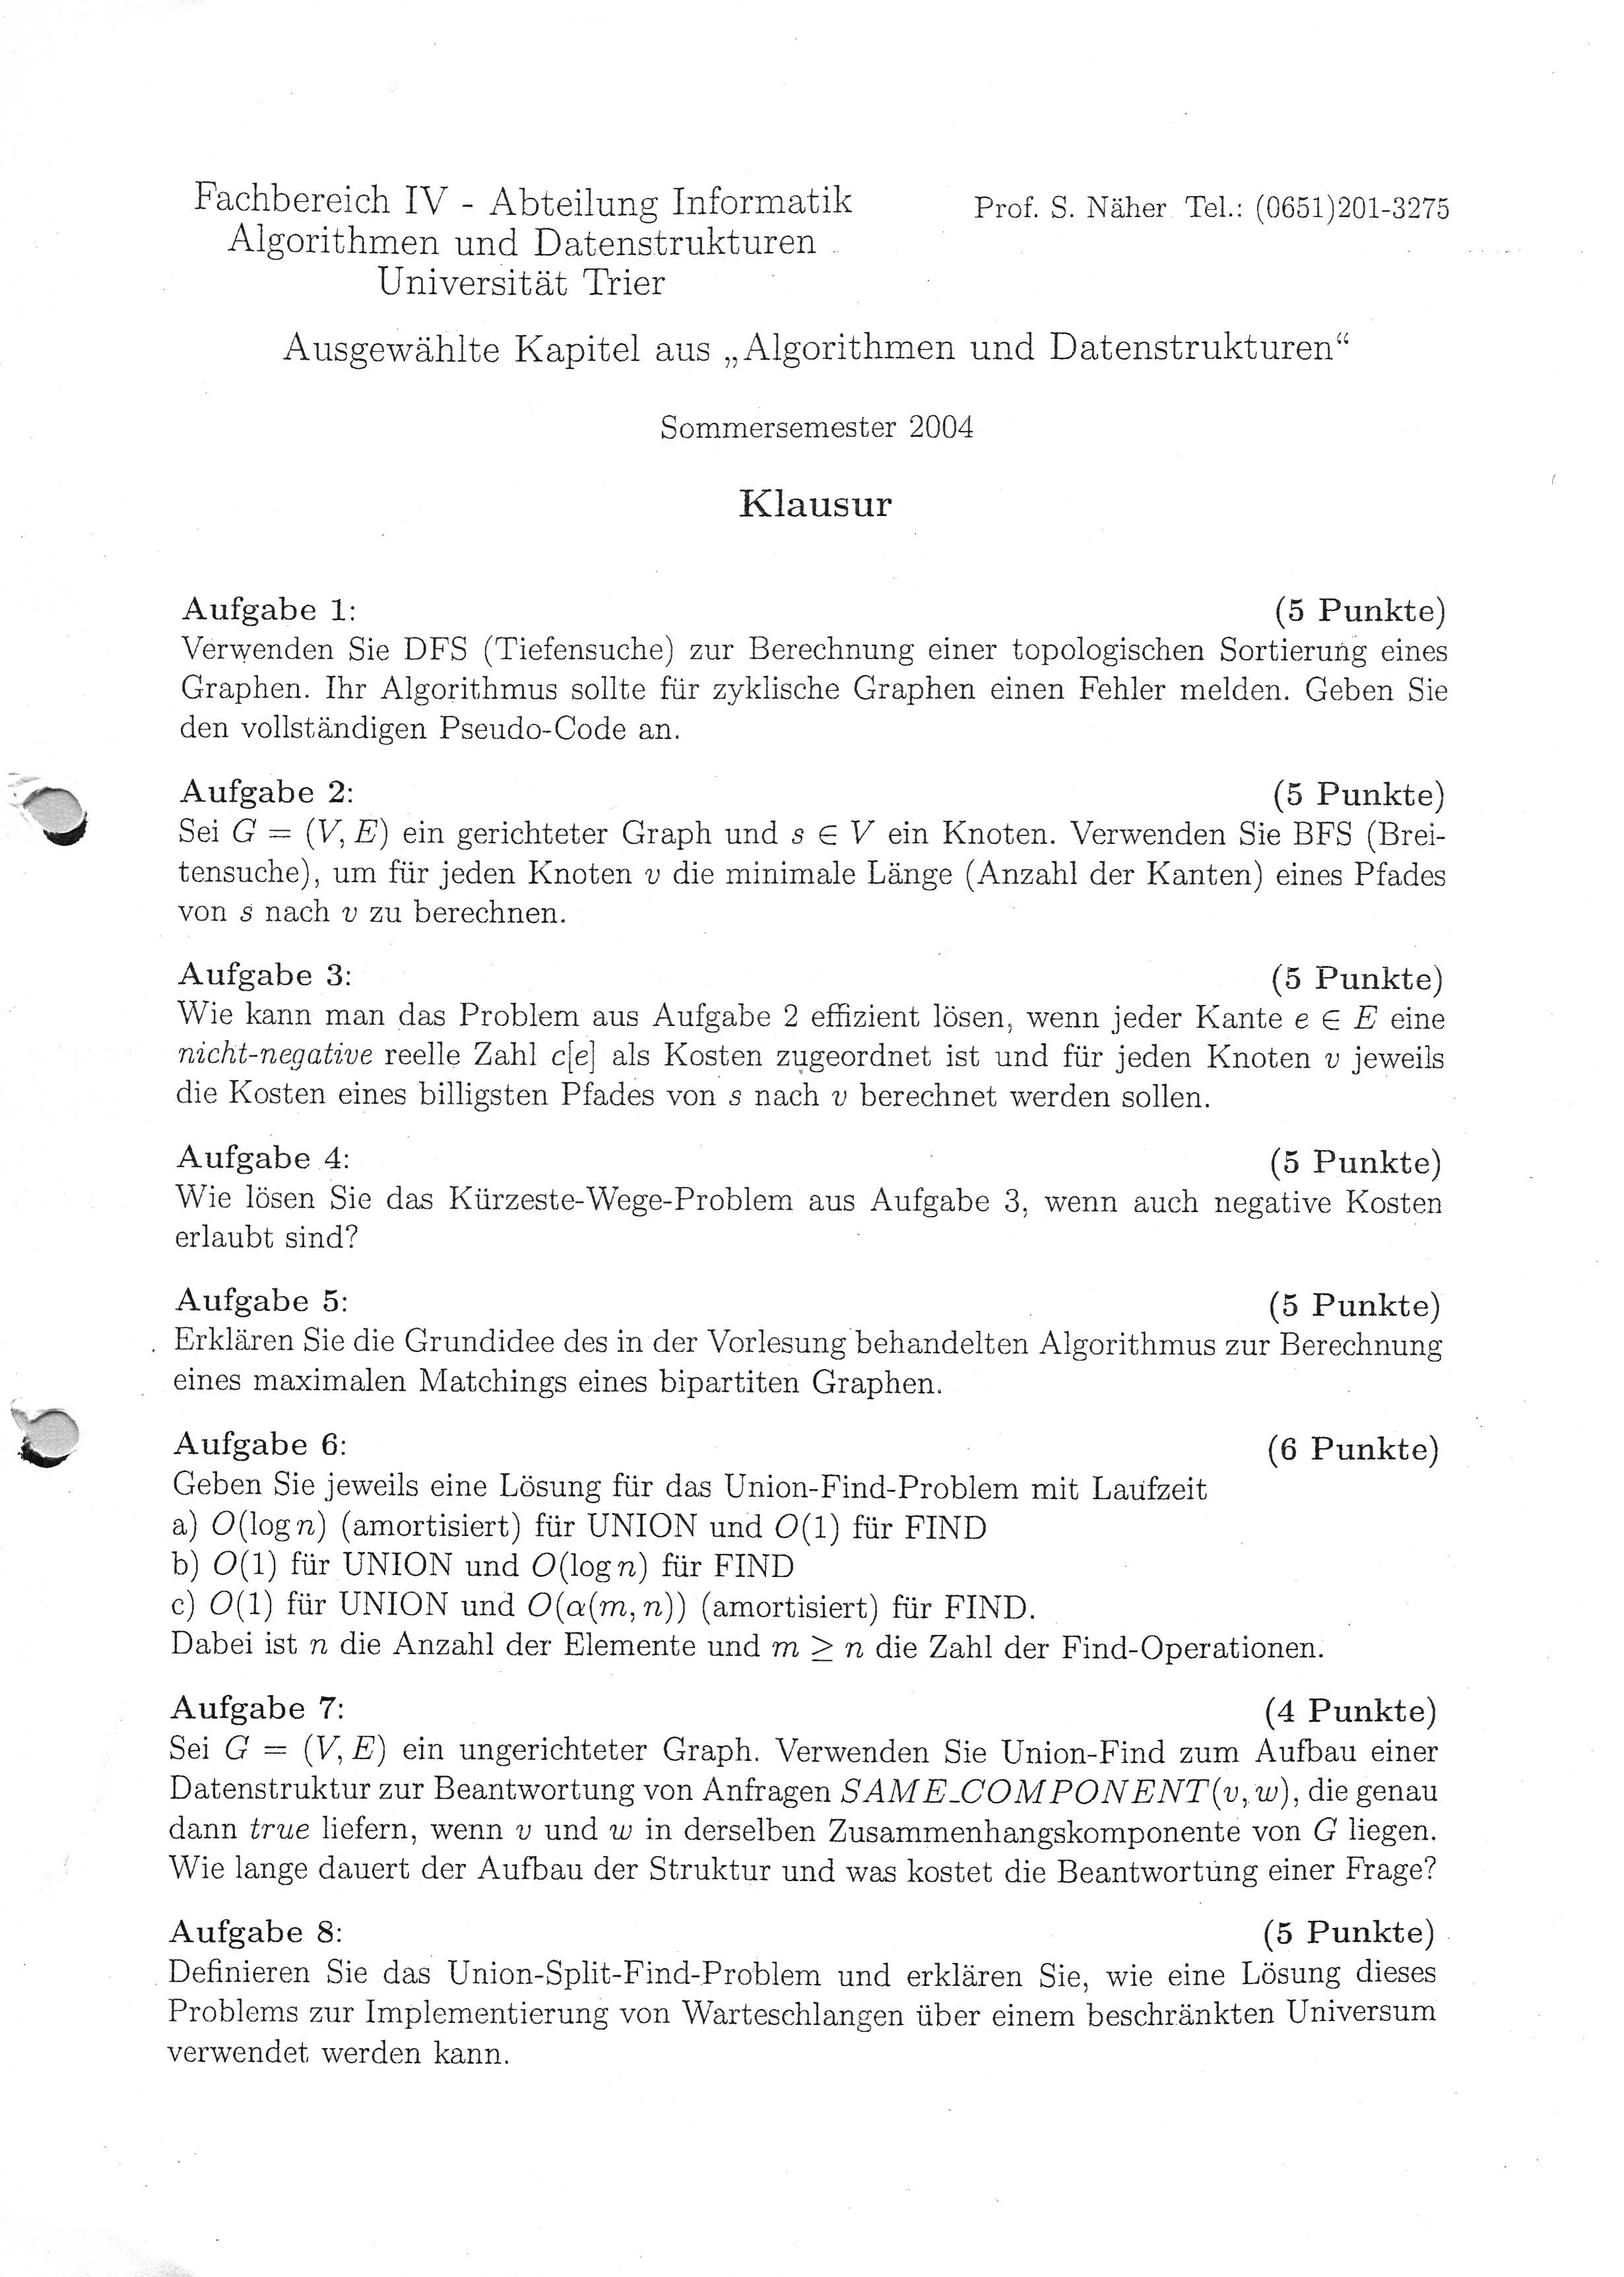
\includegraphics[]{Altklausuren/SS_2004.jpg}
	}
\end{center}

\end{document}